\documentclass[compress,red]{beamer}

\mode<presentation> {
	\usetheme{Warsaw}
}

%\beamertemplateballitem
\beamertemplateshadingbackground{gray!15}{white!15}
%\usecolortheme{crane}

% Import innych pakietow
\usepackage[utf8x]{inputenc}
\usepackage[MeX]{polski}
\usepackage{graphicx} 
\usepackage{listings}
\usepackage{amsmath}
\usepackage{amsfonts}
\usepackage{amssymb}
\usepackage{subfig}
\usepackage{verbatim}
\usepackage{algorithmic}		% Pseudokod
\usepackage{algorithm}

% USTAWIENIA PAKIETU LISTINGS
\lstloadlanguages{C}
\lstset{%
	language=C,% 
	numbers=none,%
	tabsize=4,%
	frame=single,%
	breaklines=true%
	}

% FullScreen w PDF'ach
%\hypersetup{pdfpagemode=FullScreen}


% Autor, Tytul itp.

\author{Marcin Chwedczuk \and Gleb Peregud}

\title{%
Całkowanie numeryczne
}

\institute{%
Wydział Matematyki i Nauk Informacyjnych\\
Politechnika Warszawska
}

\date{29 Listopad 2011}


%
% Głębokość spisu tresci
%
%\setcounter{tocdepth}{1} 

% Dodaj table of contents na poczatek 
% kazdej SUBsekcji
%\AtBeginSection[]
%{
%  \begin{frame}<beamer>{Agenda}
%    \tableofcontents[currentsection,currentsubsection]
%  \end{frame}
%}

% Poczatek prezentacji

\begin{document}
    \begin{frame}
        \titlepage
    \end{frame}

	%\begin{frame}{Agenda}
	%	\tableofcontents
	%\end{frame}

\section{Wstęp}

	\begin{frame}
		\frametitle{Przypomnienie - Własności całek}

	    Niech $f, g: \mathbb{R} \rightarrow \mathbb{R}$ będą funkcjami całkowalnymi
	    w sensie Riemanna, niech F będzie funkcją pierwotną $f$ ($F' = f$), 
	    ponadto niech $c \in \mathbb{R}$ 
	    wtedy zachodzą następujące równości:
	    
	    \[ \int_a^b f = F(b) - F(a) \]
	    \[ \int_a^b f = - \int_b^a f \]
	    
	    \[ \int_a^b f + g  = \int_a^b f + \int_a^b g \]
	    \[ \int_a^b cf = c \int_a^b f \]
	\end{frame}
	
	\begin{frame}
		\frametitle{Przypomnienie - Własności całek}

		\begin{figure}
	    	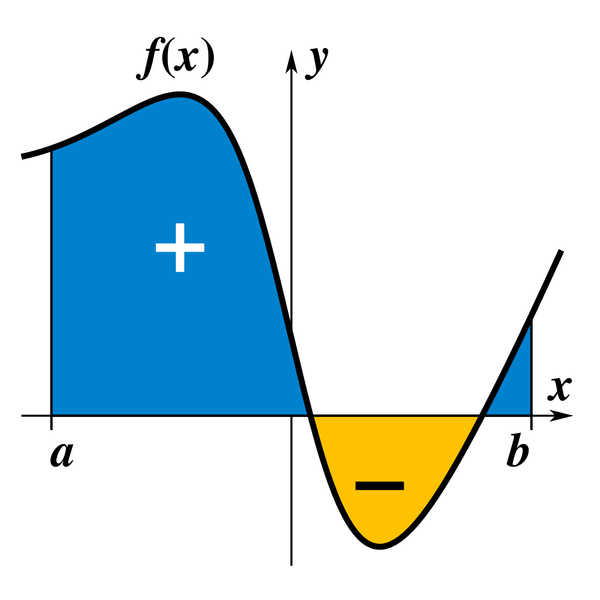
\includegraphics[scale=0.8]{./img/integration_idea_2}
	    \end{figure}
	    
	    Okazuje się że całka oznaczona z funkcji $f$ na przedziale
	    $[a, b]$ odpowiada polu figury ograniczonej przez proste
	    $x = a$ oraz $x = b$, wykres funkcji $f$ oraz oś X.
	    Przy czym pole figury leżące pod osią X uznajemy za "ujemne" 
	\end{frame}

	\begin{frame}
		\frametitle{Idea algorytmów całkowania numerycznego}
		\begin{itemize}
			\item
			 	Zamiast obliczać wartość całki z funkcji $\int_a^b f$ obliczmy pole 
			 	figury którą tworzy wykres funkcji $f$ z osią X
			 \item
			 	Pole to obliczymy dzieląc przedział całkowania $[a, b]$ na
			 	wiele wąskich "pasków"
			 \item
			 	Oszacujemy pole każdego z tych "pasków" korzystając z 
			 	wartości funkcji $f$ w kilku (niekoniecznie krańcowych) wybranych
			 	punktach - dalej będziemy te punkty nazywać węzłami
			 \item
			 	Przekształcenia które na podstawie wartości funkcji w węzłach
			 	pozwalają obliczyć pole wycinka nazywamy \textbf{kwadraturami prostymi}
			 	lub \textbf{formułami prostymi}
		\end{itemize}
	\end{frame}
	
	\begin{frame}
		\frametitle{Idea algorytmów całkowania numerycznego}
		\begin{figure}
			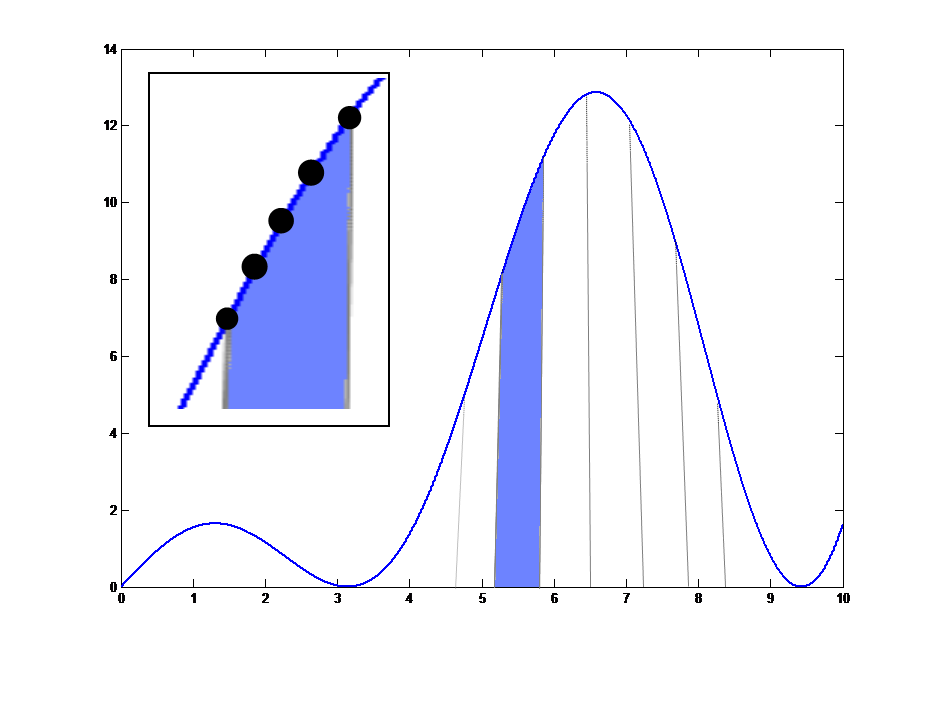
\includegraphics[scale=0.3,trim=1cm 1cm 1cm 1cm,clip]{./img/integration_idea}
			\caption{Wykres funkcji $f(x) = x + x\cos(x)$}
		\end{figure}
	\end{frame}	
	
	\begin{frame}
		\frametitle{Oznaczenia, Formuły złożone otwarte i zamknięte}
		\begin{figure}
			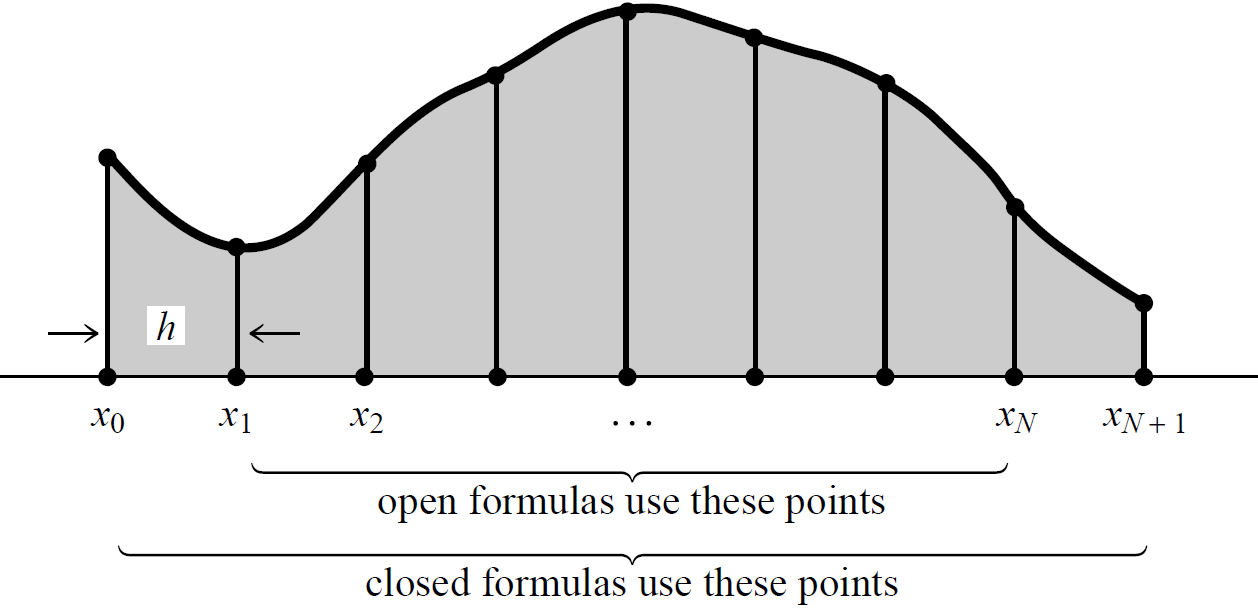
\includegraphics[scale=0.2]{./img/points}
		\end{figure}
		\only<1> {
			\begin{itemize}
				\item
					Formuły proste możemy dodawać do siebie, otrzymamy w ten 
					sposób formuły złożone pozwalające obliczyć wartość całki na
					całym przedziale $[a, b]$
			\end{itemize}
		}
		\only<2> {
			Przyjmijmy następujące oznaczenia:
			\begin{itemize}
				\item $f$ - funkcja podcałkowa
				\item $[x_0, x_{N+1}]$ - przedział całkowania
				\item $ x_i = x_0 + ih, \ i = 0, 1, \ldots, N+1 $
				\item $ f_i = f(x_i) $
			\end{itemize}
		}
	\end{frame}
	
\section{Kwadratury proste}
	
	\begin{frame}
		\frametitle{Kwadratury Newtona-Cotes'a - Kwadratura trapezów}
		\[ \int_{x0}^{x1} f = \frac{h}{2}(f_0 + f_1) + O(h^3 f'') \]
		\begin{figure}
			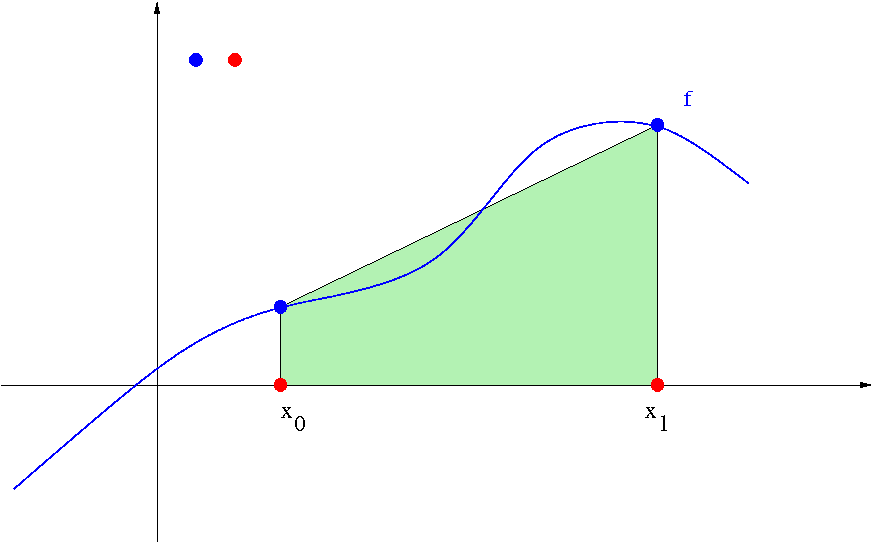
\includegraphics[scale=0.3]{./img/q_trap}
		\end{figure} 
	\end{frame}	
	
	\begin{frame}
		\frametitle{Kwadratury Newtona-Cotes'a - Kwadratura Simpsona}
		\[ \int_{x0}^{x2} f = \frac{h}{3}(f_0 + 4f_1 + f_2) + O(h^5 f^{(4)}) \]
		\begin{figure}
			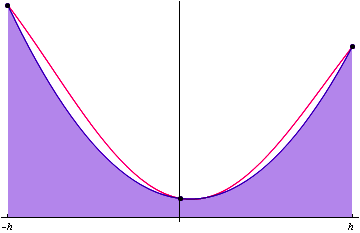
\includegraphics[scale=0.5]{./img/q_sim}
		\end{figure} 
	\end{frame}	
	
	\begin{frame}
		\frametitle{Kwadratury Newtona-Cotes'a}
		Dwie pozostałe kwadratury mają znaczenie czysto teoretyczne...
		\\[1cm]
		
		Kwadratura Simpsona 3/8
		\[ \int_{x0}^{x3} f = \frac{h}{8}(3f_0 + 9f_1 + 9f_2 + 3f_3) + O(h^5 f^{(4)}) \]
		
		Kwadratura Bode'a
		\[ \int_{x0}^{x4} f = \frac{h}{45}(14f_0 + 64f_1 + 24f_2 + 64f_3 + 14f_4) + O(h^7 f^{(6)}) \]
	\end{frame}	
	
	\begin{frame}
		\frametitle{Formuły ekstrapolacyjne} 
		\begin{itemize}
			\item
				Poprzednio przedstawione formuły pozwalają nam dokonać
				całkowania na dowolnym przedziale zamkniętym $[a, b]$
			\item
				Niestety nie każda funkcja podcałkowa jest zdefiniowana na 
				całym przedziale np. funkcja $\frac{1}{x}$ nie jest zdefiniowana 
				w punkcie $x = 0$, a zatem stosując poprzednie formuły nie możemy 
				obliczyć $\int_0^1 \frac{1}{x} dx$
			\item
				Dalej założymy że funkcja nie jest definiowana w punkcie $ x_0 $,
				natomiast jest definiowana w punktach $ x_1, \ldots, x_n $
		\end{itemize}
	\end{frame}	
	
	\begin{frame}
		\frametitle{Formuły ekstrapolacyjne} 
		\begin{itemize}
			\item
				Wartość całki w przedziale $[x_0, x_1]$ postaramy się oszacować
				za pomocą wartości funkcji w punktach $ x_1, \ldots, x_n $
		\end{itemize}
		
		\[ \int_{x0}^{x1} f = h f_1 + O(h^2 f') \]
		\[ \int_{x0}^{x1} f = \frac{h}{2} (3f_1 - f_2) + O(h^3 f'') \]
		\[ \int_{x0}^{x1} f = \frac{h}{12} (23f_1 - 16f_2 + 5f_3) + O(h^4 f^{(3)}) \]
	\end{frame}
	
\section{Kwadratury złożone}
	
	\begin{frame}
		\frametitle{Kwadratura trapezów}
		
		\[ \int_{x_0}^{x_{N+1}} f = h \left[ \frac{1}{2}f_0 + f_1 + f_2 + \ldots
		 + f_{N} + \frac{1}{2}f_{N+1} \right] + O(\frac{1}{N^2})\]
		 
		 \begin{figure}
		 	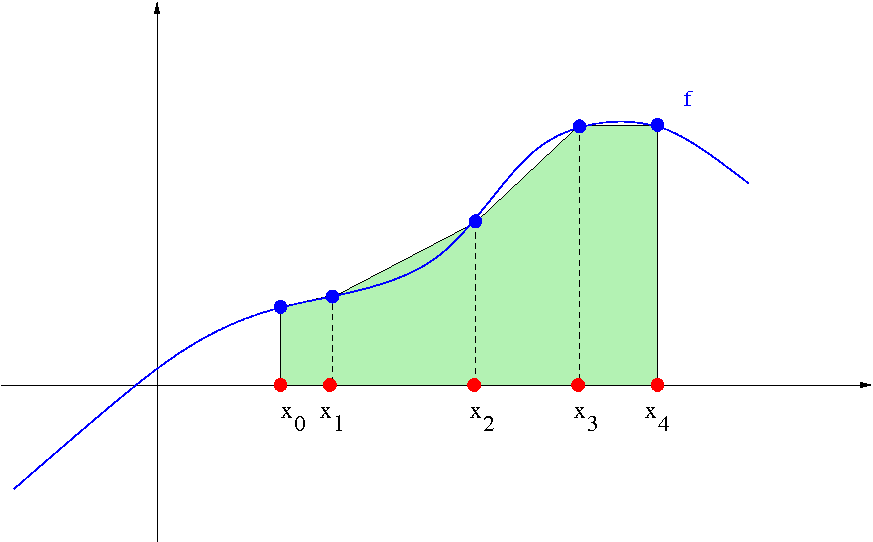
\includegraphics[scale=0.2]{./img/q_trap2}
		 	\caption{Poprzez wielokrotne zastosowanie prostej kwadratury trapezów do 
		pod przedziałów $[x_i, x_{i+1}]$ otrzymujemy złożoną kwadraturę trapezów}
		 \end{figure}
	\end{frame}	
	
	\begin{frame}
		\frametitle{Kwadratura Simpsona}
		
		\[
		\int_{x_0}^{x_{N+1}} f = h \left[ \frac{1}{3}f_0 + \frac{4}{3}f_1 + \frac{2}{3}f_2 +  \ldots +\frac{4}{3}f_N + \frac{1}{3}f_{N+1} \right]
		 + O(\frac{1}{N^4})\]

		 \begin{figure}
		 	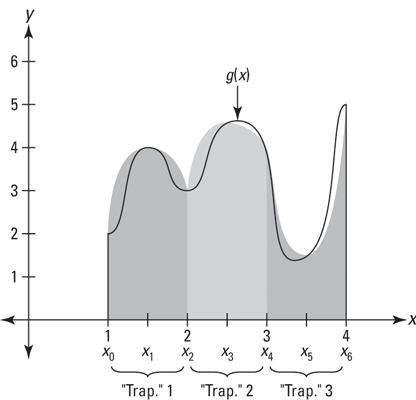
\includegraphics[scale=0.3]{./img/q_sim2}
		 	\caption{Poprzez wielokrotne zastosowanie reguły Simpsona do 
		pod przedziałów $[x_i, x_{i+1}]$ otrzymujemy rozszerzoną regułę Simpsona}
		 \end{figure}
	\end{frame}	
	
	\begin{frame}
		\frametitle{Złożone formuły otwarte}
		
		Otwarta formuła bazująca na kwadraturze trapezów
		\[
		\int_{x_0}^{x_{N+1}} f = h \left[ \frac{3}{2}f_1 + f_2 +  \ldots + f_{N-1} + \frac{3}{2}f_{N} \right]
		 + O(\frac{1}{N^2})\]

		Otwarta formuła bazująca na regule Simpsona
		\begin{figure}
			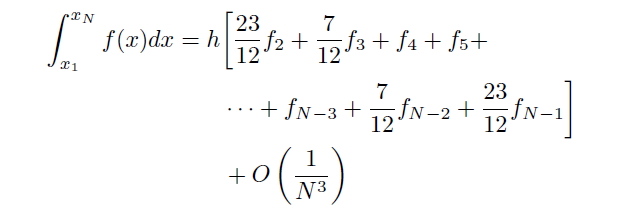
\includegraphics[scale=0.5]{./img/ex_sim}
		\end{figure}
	\end{frame}	
	
	\begin{frame}
		\frametitle{Złożone formuły otwarte}
		
		Kwadratura prostokątów (kwadratura punktu środkowego)
		\[
		\int_{x_0}^{x_{N+1}} f = h \left[ f_\frac{1}{2} + f_\frac{3}{2} +  \ldots + f_\frac{N-2}{2} + f_\frac{N}{2} \right]
		 + O(\frac{1}{N^2})\]

		\begin{figure}
			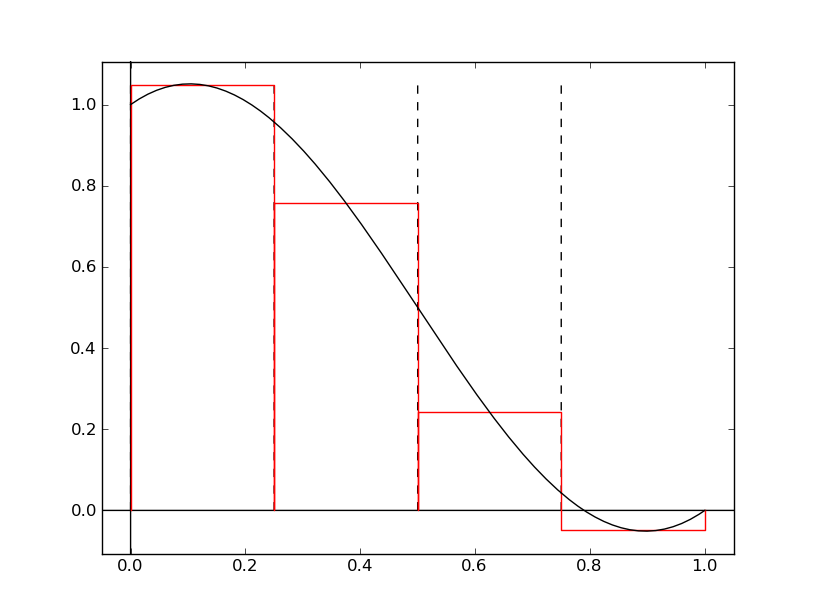
\includegraphics[scale=0.3]{./img/q_rect2}
		\end{figure}
	\end{frame}	
	
\section{Algorytmy}	
% Algorytm przyrostowy na trapezy i roberga (koniecznie bo jest ciekawy)
% Jak Ci się bedzie nudzilo to  mozesz Simpsona dodac
	
\section{Całki niewłaściwe}
% Tylko teoria - tj. to przeksztalcenie z niewlasciwej na wlasciwa
	
\section{Całki wielowymiarowe}
% Zamiana calki wielowymiarowej na iterowane + mozesz
% cos dodac od siebie

% Jesli chcesz zebym to ja cos dodal ewentulanie wyrzucil
% to pisz email postaram sie odpowiedziec w przeciagu 1h
% w Zasadzie jedyne co mozemy jeszcze dorzucic to MonteCarlo
% ewentualnie prosty przyklad z kwadraturami gaussa

\section{Zakończenie}
	% Mały żart na koniec ???
	\begin{frame}
		\frametitle{THE END}
		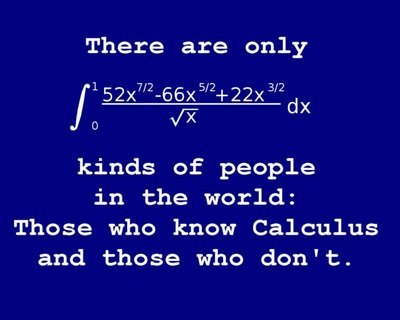
\includegraphics[scale=0.7]{./img/calculus}
	\end{frame}
	
	\begin{frame}
		\frametitle{Bibliografia}
		\begin{itemize}
			\item Press, Teukolsky, Vetterling, Flannery
			\textit{Numerical Recipes in C. The Art of Scientific Computing}
			Wydanie drugie
		\end{itemize}
	\end{frame}	
	
	\begin{frame}
		\frametitle{Zakończenie}
		\only<1>{		
		\begin{Huge}
			Pytania ?
		\end{Huge}}
		\only<2>{
		\begin{Huge}
			Dziękujemy za uwagę
		\end{Huge}
			}
	\end{frame}

\end{document}
